%%%%% Diagnosing Thoracic Diseases Using Machine Learning & Medical Imaging

\documentclass{article}

\usepackage{microtype}
\usepackage{graphicx}
\usepackage{subfigure}
\usepackage{subcaption}
\usepackage{caption}
\usepackage{booktabs}
\usepackage[%  
    colorlinks=true,
    pdfborder={0 0 0},
    linkcolor=red
]{hyperref}

\newcommand{\theHalgorithm}{\arabic{algorithm}}
\usepackage[accepted]{icml2024}

\usepackage{amsmath}
\usepackage{amssymb}
\usepackage{mathtools}
\usepackage{amsthm}

\usepackage[capitalize,noabbrev]{cleveref}

\graphicspath{{./Images}}

%%%%%%%%%%%%%%%%%%%%%%%%%%%%%%%%
% THEOREMS
%%%%%%%%%%%%%%%%%%%%%%%%%%%%%%%%
\theoremstyle{plain}
\newtheorem{theorem}{Theorem}[section]
\newtheorem{proposition}[theorem]{Proposition}
\newtheorem{lemma}[theorem]{Lemma}
\newtheorem{corollary}[theorem]{Corollary}
\theoremstyle{definition}
\newtheorem{definition}[theorem]{Definition}
\newtheorem{assumption}[theorem]{Assumption}
\theoremstyle{remark}
\newtheorem{remark}[theorem]{Remark}

\usepackage[textsize=tiny]{todonotes}

\icmltitlerunning{Diagnosing Thoracic Diseases Using ML}

\begin{document}

\twocolumn[
\icmltitle{Diagnosing Thoracic Diseases Using Machine Learning and Medical Imaging}

\begin{icmlauthorlist}
\icmlauthor{Wendy Carvalho (02026116),}{}
\icmlauthor{Meriem Elkoudi (02015993),}{}
\icmlauthor{Chris Peters (01989716),}{}
\icmlauthor{Saim Siddiqui (02018510),}{}
\icmlauthor{and Amitha Thalanki (02077527)}{}
\end{icmlauthorlist}

\vskip 0.3in
]

\begin{abstract}
    \textbf{TODO: Write a concise summary of the project and the conclusions of the work. It should be no longer
    than one short paragraph (e.g. 200 words).}
\end{abstract}

\section{Introduction}
Thoracic diseases, including pneumonia, emphysema, and fibrosis, are common causes of morbidity and
mortality worldwide. Chest X-rays are one of the most widely accessible and commonly used diagnostic
tools for detecting these conditions. However, interpreting these images is complex, and clinical
diagnoses are often challenging, even for experienced radiologists.

Machine learning techniques are used to address this challenge by enabling automated analysis of
medical images. Bringing this leading-edge technology's immense power into the diagnostics field can
potentially increase the capacity for trained professionals to diagnose patients properly, sooner,
and in more difficult-to-identify cases.

This project aims to build a computer-aided diagnostic (CAD) tool capable of diagnosing thoracic
diseases from chest X-ray images, assisting clinicians by automating the detection of common thoracic
diseases. This has been implemented using Support Vector Machines (SVM) and Convoluted Neural Networks
(CNN) in the form of ResNet50 and MobileNet. The efficacy of all are tested.

\section{Data}
\textbf{TODO: Describe the data used for experiments and report data statistics as well as interesting
observations or patterns in the data.}

The data for this project has been obtained from the NIH ChestX-ray8 dataset, an open-source,
hospital-scale collection of medical images, which will be essential for developing a CAD system.
The original NIH ChestX-ray8 dataset contains 108,948 images from 32,717 patients, however, the
labels are frequently incorrect and misdiagnoses.
A subset of 810 images was chosen based on the evaluation of radiologists themselves. The 810 image
subset is the only commonly known verified chest x-ray dataset. 

The data can be classified into 14 different labels, with the capability of multi-label classification.
The "None" label is also a possibility, but only occurs in the absence of any diseases and cannot be
combined with any other label. The 14 possible abnormal labels are: 
\begin{itemize}
    \item Hernia,
    \item Pleural Thickening,
    \item Fibrosis,
    \item Emphysema,
    \item Edema,
    \item Consolidation,
    \item Pneumothorax,
    \item Pneumonia,
    \item Nodule,
    \item Mass,
    \item Infiltration,
    \item Effusion,
    \item Cardiomegaly,
    \item and Other.
\end{itemize}

In Figure \ref{fig:normalvabnormal}, the dataset's distribution of normal and abnormal x-rays is shown,
where abnormal is any image with at least one of the 14 aforementioned labels, and where
normal is any image with the "None" label. The abnormal category outnumbers the normal category quite
a bit, which may contribute to the class imbalance.

%%% NORMAL VS ABNORMAL FIGURE %%%
\begin{figure}[!h]
    \centering
    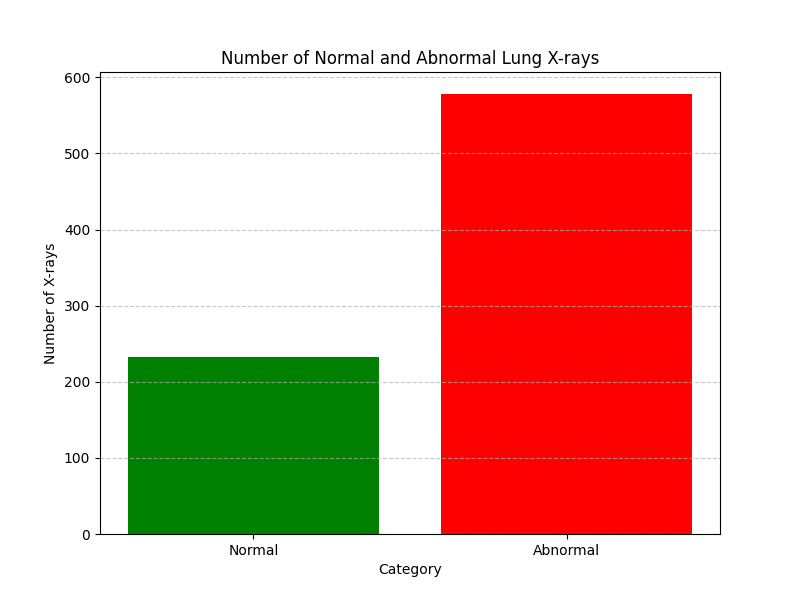
\includegraphics[scale=0.405]{normal_vs_abnormal}
    \caption{The distribution of normal vs. abnormal lung x-rays}
    \label{fig:normalvabnormal}
\end{figure}

As shown in Figure \ref{fig:datasetdistribution}, there is a very clear class imbalance, with "None"
and "Effusion" occuring the most and "Pneumonia" and "Hernia" occuring the least. 

%%% DATASET DISTRIBUTION FIGURE -- wide image, so must appear across both columns %%%
\begin{figure*}[!h]
    \centering
    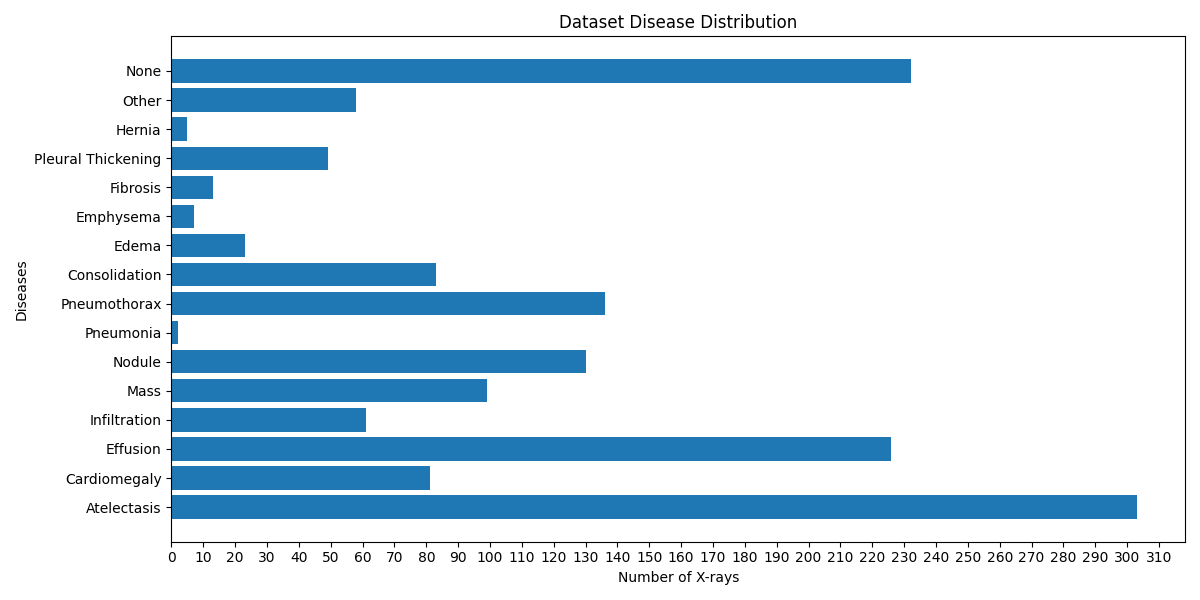
\includegraphics[scale=0.55]{disease_distr}
    \caption{The disease distribution of the dataset with Diseases vs. Number of x-rays.
    As shown, there are 15 labels, including the "None" label. The class imbalance can also be seen.}
    \label{fig:datasetdistribution}
\end{figure*}

\section{Methods}
\textbf{TODO: Provide a detailed description of your method and explain why the method is a good fit for
the problem.}

\section{Results}
\textbf{TODO: Briefly describe the evaluation approach and metrics. Report performance metrics for the method(s) through Figures or Tables.
Report insights obtained from the results. Good ways to obtain insight are ablation analysis, error
analysis, and use of synthetic data.}

\section{Conclusion}
\textbf{TODO: In one short paragraph concisely summarize the main points and insights of the project,
describe potential directions to extend your project, and describe limitations of your project.}

\section{Contribution Chart}
\textbf{TODO: Complete the following Table to clearly report the contributions that each team
member made to the final project. (Task/Subtask, Student ID, Commentary on Contribution)}

\begin{table}[!h]
    \centering
    \begin{tabular}{| c || c | c | c |}
        \hline
        & Student ID & Task & Commentary on Contribution \\
        \hline
        Name & & & \\
        \hline
        Name & & & \\
        \hline
        Name & & & \\
        \hline
        Name & & & \\
        \hline
        Name & & & \\
        \hline
    \end{tabular}
\end{table}
%%% TO DO: ADD BIBLIOGRAPHY AND RESOURCES %%%
\end{document}
